\subsubsection{Class Diagram}

\begin{figure}[H]
	\centering
	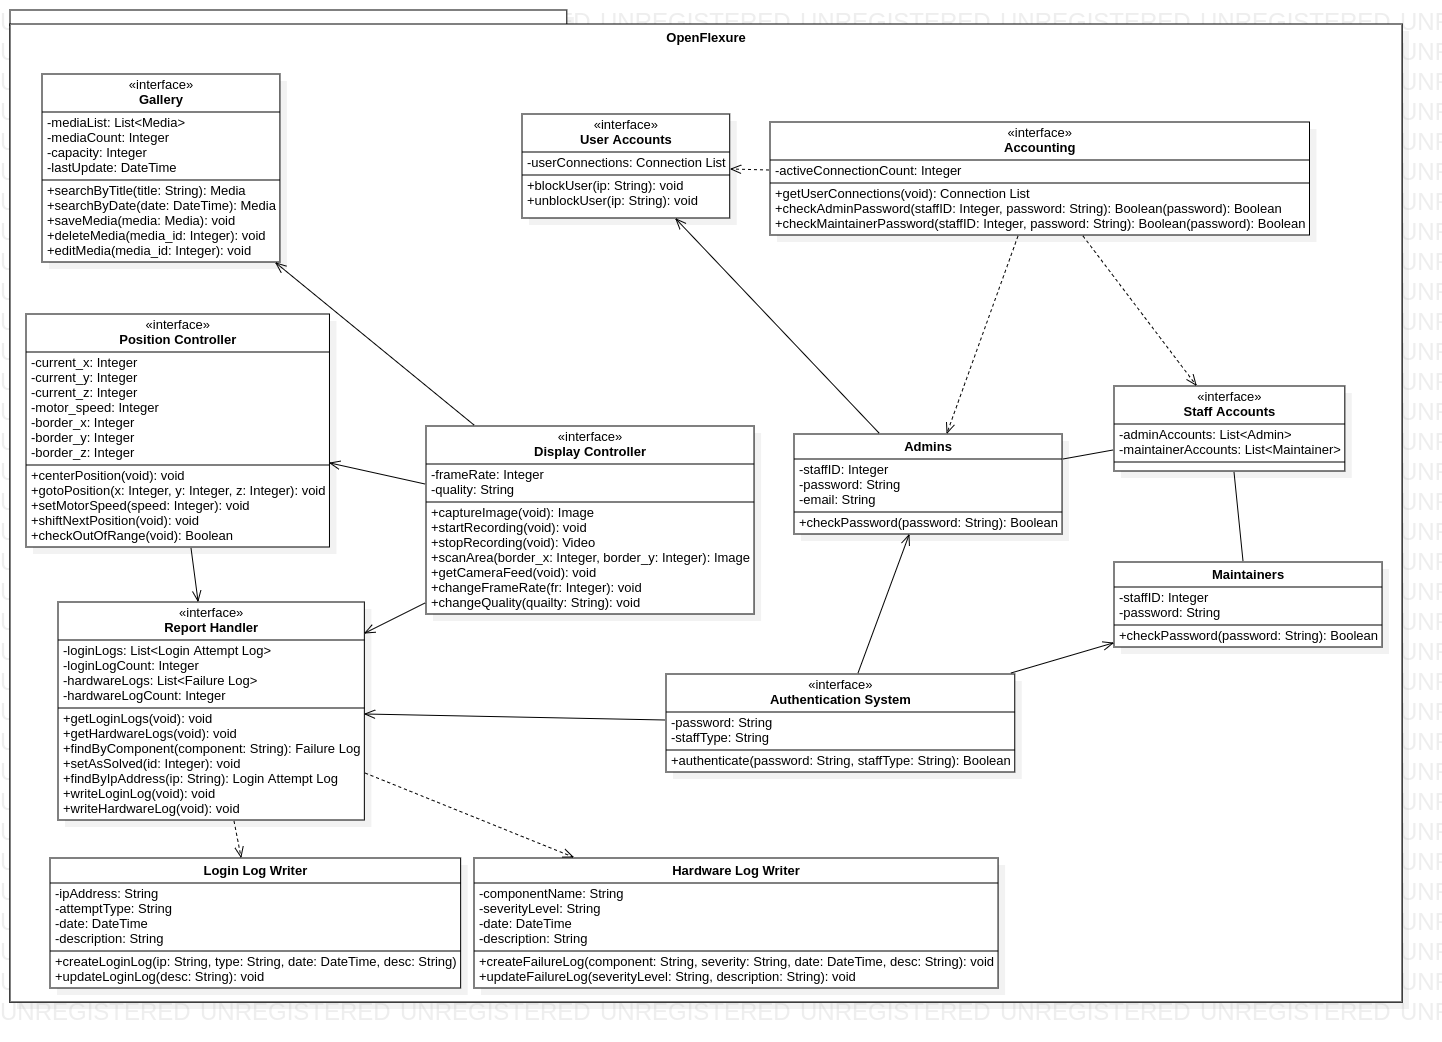
\includegraphics[scale=0.3]{Uml_Images/interface_class_diagram}
	\caption{Interface Class Diagram for OpenFlexure}
	\label{fig:interface_class_diagram}
\end{figure}

\begin{table}[H]
	\centering
	\begin{tabular}{|l|C|}
		\hline
		\textbf{Operation}   &  \textbf{Description}\\
		\hline
		searchByTitle   &  returns the media with given title\\
		\hline
		searchByDate   &  returns the media with given date\\
		\hline
		saveMedia  &  saves the given media to the gallery media list\\
		\hline
		deleteMedia   &  delete the media with given id from the gallery media list\\
		\hline
		editMedia   &  edits the media with given id\\
		\hline
		centerPosition   &  positions the stage to the center\\
		\hline
		gotoPosition   &  positions the stage to the point with the given coordinates\\
		\hline
		setMotorSpeed  &  sets the motor speed\\
		\hline
		shiftNextPosition  &  shifts the stage position to the next one by incrementing the current coordinates\\
		\hline
		checkOutOfRange  &  checks if the current coordinates are out of range\\
		\hline
		captureImage  &  captures the displayed livestream and returns the captured image\\
		\hline
		startRecording   &  starts recording the livestream\\
		\hline
		stopRecording   &  stops the ongoing recording and returns the recorded video\\
		\hline
		scanArea & scans the area with the given border coordinates and returns it as image\\
		\hline
		getCameraFeed & streams the live camera feed \\
		\hline
		changeFrameRate & changes the frame rate of the camera\\
		\hline
		changeQuality & changes the quality of the camera\\
		\hline
		getLoginLogs & returns the list of Login Attempt Logs\\
		\hline
		getHardwareLogs & returns the list of Failure Logs\\
\hline
		findByComponent & returns the Failure Log with the given component name\\
\hline
		setAsSolved & sets the status of the log with given id as solved\\
\hline
		findByIpAddress & returns the Login Attempt Log with the given component name\\
\hline
		writeLoginLog & writes the login log created by Login Log Writer to the loginLogs list\\
\hline
		writeHardwareLog & writes the hardware log created by Hardware Log Writer to the hardwareLogs list\\
\hline
		createLoginLog & creates a Login Attempt Log and fills it with the given parameters\\
\hline
	\end{tabular}
\end{table}

\begin{table}[H]
	\centering
	\begin{tabular}{|l|C|}
		\hline
	updateLoginLog & updates the Login Attempt Log with the given id\\
	\hline
	createFailureLog & creates a Failure Log and fills it with the given parameters\\
	\hline
	updateFailureLog & updates the Failure Log with the given id\\
	\hline
	authenticate & checks the password of the user with given staff type and authenticates him/her\\
	\hline
	getUserConnections & returns the list of Connections \\
	\hline
	checkAdminPassword & compares the given password with the password of the admin with given staffID and returns the result of the comparison \\
	\hline
	checkMaintainerPassword & compares the given password with the password of the maintainer with given staffID and returns the result of the comparison \\
	\hline
	blockUser & sets the blockStatus of the user with the given ip as True \\
	\hline
	unblockUser & sets the blockStatus of the user with the given ip as False \\
	\hline
	checkPassword & compares the given password with the password of the admin/maintainer \\
	\hline
	\end{tabular}
	\caption{Operation Descriptions}
	\label{tab:operation_descriptions}
\end{table}

\begin{figure}[H]
	\centering
	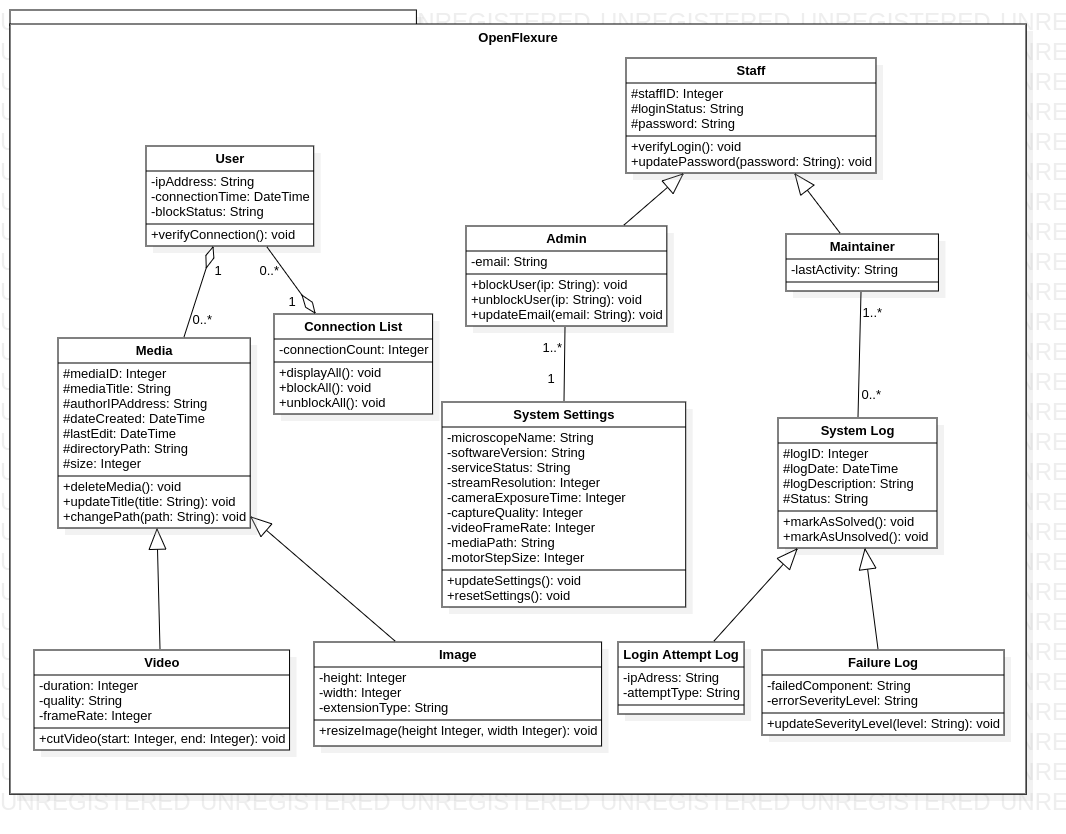
\includegraphics[scale=0.4]{Uml_Images/db_class_diagram}
	\caption{Database Class Diagram for OpenFlexure}
	\label{fig:db_class_diagram}
\end{figure}

\subsubsection{Database Operations}
\begin{table}[H]
	\centering
	\begin{tabular}{|p{5cm}|p{7cm}|}
		\hline
		\textbf{Operation} & \textbf{CRUD Operations} \\
		\hline
		verifyLogin &
		CREATE:\newline
		READ: \texttt{Staff} \newline
		UPDATE: \texttt{Staff} \newline
		DELETE: \\
		\hline
		updatePassword &
		CREATE:\newline
		READ: \newline
		UPDATE: \texttt{Staff}\newline
		DELETE: \\
		\hline
		updateEmail &
		CREATE:\newline
		READ: \newline
		UPDATE: \texttt{Admin}\newline
		DELETE: \\
		\hline
		blockUser &
		CREATE:\newline
		READ: \newline
		UPDATE: \texttt{User}\newline
		DELETE: \\
		\hline
		unblockUser &
		CREATE:\newline
		READ: \newline
		UPDATE: \texttt{User}\newline
		DELETE: \\
		\hline
		updateSettings &
		CREATE:\newline
		READ: \newline
		UPDATE: \texttt{Settings}\newline
		DELETE: \\
		\hline
		resetSettings &
		CREATE:\newline
		READ: \texttt{Settings}\newline
		UPDATE: \texttt{Settings}\newline
		DELETE: \\
		\hline
		markAsSolved &
		CREATE:\newline
		READ: \newline
		UPDATE: \texttt{System Log}\newline
		DELETE: \\
		\hline
	\end{tabular}
\end{table}

\begin{table}[H]
	\centering
	\begin{tabular}{|p{5cm}|p{7cm}|}
		\hline
		markAsUnsolved &
		CREATE:\newline
		READ: \newline
		UPDATE: \texttt{System Log}\newline
		DELETE: \\
		\hline
		updateSeverityLevel &
		CREATE:\newline
		READ: \newline
		UPDATE: \texttt{Failure Log}\newline
		DELETE: \\
		\hline
		verifyConnection &
		CREATE: \newline
		READ: \texttt{User}\newline
		UPDATE: \texttt{User}\newline
		DELETE: \\
		\hline
		deleteMedia &
		CREATE: \newline
		READ:  \newline
		UPDATE: \newline
		DELETE: \texttt{Media} \\
		\hline
		updateTitle &
		CREATE: \newline
		READ:  \newline
		UPDATE: \texttt{Media} \newline
		DELETE:  \\
		\hline
		changePath &
		CREATE: \newline
		READ:  \newline
		UPDATE: \texttt{Media} \newline
		DELETE:  \\
		\hline
		cutVideo &
		CREATE: \newline
		READ:  \newline
		UPDATE: \texttt{Video} \newline
		DELETE:  \\
		\hline
		resizeImage &
		CREATE: \newline
		READ:  \newline
		UPDATE: \texttt{Image} \newline
		DELETE:  \\
		\hline
		displayAll &
		CREATE: \newline
		READ: \texttt{Connection List}, \texttt{User}\newline
		UPDATE: \newline
		DELETE: \\
		\hline
	\end{tabular}
\end{table}
\begin{table}[H]
	\centering
	\begin{tabular}{|p{5cm}|p{7cm}|}
		\hline
		blockAll &
		CREATE: \newline
		READ: \texttt{Connection List} \newline
		UPDATE: \texttt{User} \newline
		DELETE: \\
		\hline
		unblockAll &
		CREATE: \newline
		READ: \texttt{Connection List} \newline
		UPDATE: \texttt{User} \newline
		DELETE: \\
		\hline
	\end{tabular}
	\caption{CRUD Operations}
	\label{tab:crud_operations}
\end{table}

\subsubsection{Design Rationale}
\paragraph{Interface Class Diagram}
\begin{itemize}
	\item Report Handler is responsible for creating and storing logs related to hardware failures and login errors.
	\item Both Display Controller and Position Controller associated with the Report Handler to report hardware related problems.
	\item Authentication System is associated with the Report Handler to report suspicious login attempts.
	\item To allow the maintainers to use View System Logs function defined in use-case diagram, Maintainers component uses the interface provided by the Report Handler.
	\item To allow the admins to use Block User and Unblock User functions defined in use-case diagram, Admins part is associated with the User Accounts part.
	\item To be able to store the captured images, scans and recorded videos, Display Controller is associated with the Gallery.
\end{itemize}
\paragraph{Database Class Diagram}
\begin{itemize}
	\item For easy and fast usability of the microscope, users do not have to authenticate to the system. Therefore, for user records, password information is omitted.
	\item To avoid repetition of the attributes, Media, System Log and Staff parent classes are defined. 
	\item To be able to handle different types of errors, Login Attempt Log and Failure Log classes are created.
	\item To allow the maintainer to use View System Logs function defined in use-case diagram, Maintainer and System Logs classes are linked to each other.
\end{itemize}